\chapter{Yen}
%

% - Purpose & Problem description:
%     These first two parts give reader short details about the test case,
%     the physical phenomena involved and specify how the numerical solution will be validated
%
\section{Purpose}
%
The purpose of this test is to assess the ability of \gaia to reproduce the bed evolution in an alluvial channel bend under unsteady-flow conditions.
The mechanics of sediment transport in channel bends, frequently appearing in natural rivers, are much more complex than that in straight channels.
The complexity is twofold: on the one hand, the sediment transport in a channel bend is subject not only to longitudinal transport,
but also to transverse transport and transverse sorting by the secondary flow inherently associated with bends.
On the other hand, the unsteadiness of flow in natural rivers certainly has some effects on the structure of the flow field,
thereby affecting the motion of sediment particles.

This test is the experimental setup (RUN 4) proposed by Yen and Lee (1995).
In this case, the bed evolution of a 180$^{\circ}$ channel bed with an initial flat bottom is computed for a triangular-shaped $300$ min. hydrograph.
Numerical results are validated by measured contours of bed evolution after at the end of the experience and by measured bottom elevations at
two different cross sections (90$^{\circ}$ and 180$^{\circ}$). This validation case can be performed for uniform or graded sediment distribution.
There are several cases in this example. With graded sediments all implemented bedload formulas (except one because it needs waves) and hiding formulas are tested. With uniform sediments all implemented slope formulations are tested.
Since only the sediment diameters are variable, the results with 1 class or with 5 classes can all be compared to the experimental data.
An additional test was added to test the keyword \telkey{SPINUP TIME FOR BED UPDATING}. In this test, a run with bed load and suspended load is executed, with a hydrodynamic spinup time of 12 minutes.
%
\section{Problem setup}
%
The flume consists of a straight section of $11.5$ m long, a $180^{\circ}$ bend of $4.0$ m radius and a downstream straight section of
$11.5$ m long, with a constant slope in flow direction equal to $0.002$. The width of the flume channel is $1.0$ m.
A triangular-shaped inflow hydrograph with an initial discharge of $Q=0.02$ m$^3/$s, a water depth at the outflow of $h = 0.0544$ m
and a peak discharge of equal to $0.053$ m$^3/$s (water depth $h=0.103$m) at $T = 100$ min
is used, see Figure~\ref{fig:hydro}. After $T = 100$ min, the inflow discharge is reduced linearly until
it reached the initial values at the end of the experiment ($T = 300$ min).

The sediment is characterized by a median diameter of $D_{50}=1$ mm. This value is used for the case uniform sediment.
For the case graded sediment, five sediment classes with diameters $D=0.31, 0.64, 1.03, 1.69$ and $3.36$ mm are chosen to
reproduce the sediment distribution of the experiment. For this case, an initial distribution of 20\% for each class is adopted.
All implemented bedload transport formulas are tested as well as all slope effect formulas. The secondary currents correction are accounted for this test.
The default value of $\alpha=1$ is used for the secondary currents parameter, therefore the Engelund parameter $A=7$.
For the case graded sediment, two vertical sediment layers with a total thickness equal to $20$ cm are assumed.

\begin{figure}[!h]
\centering
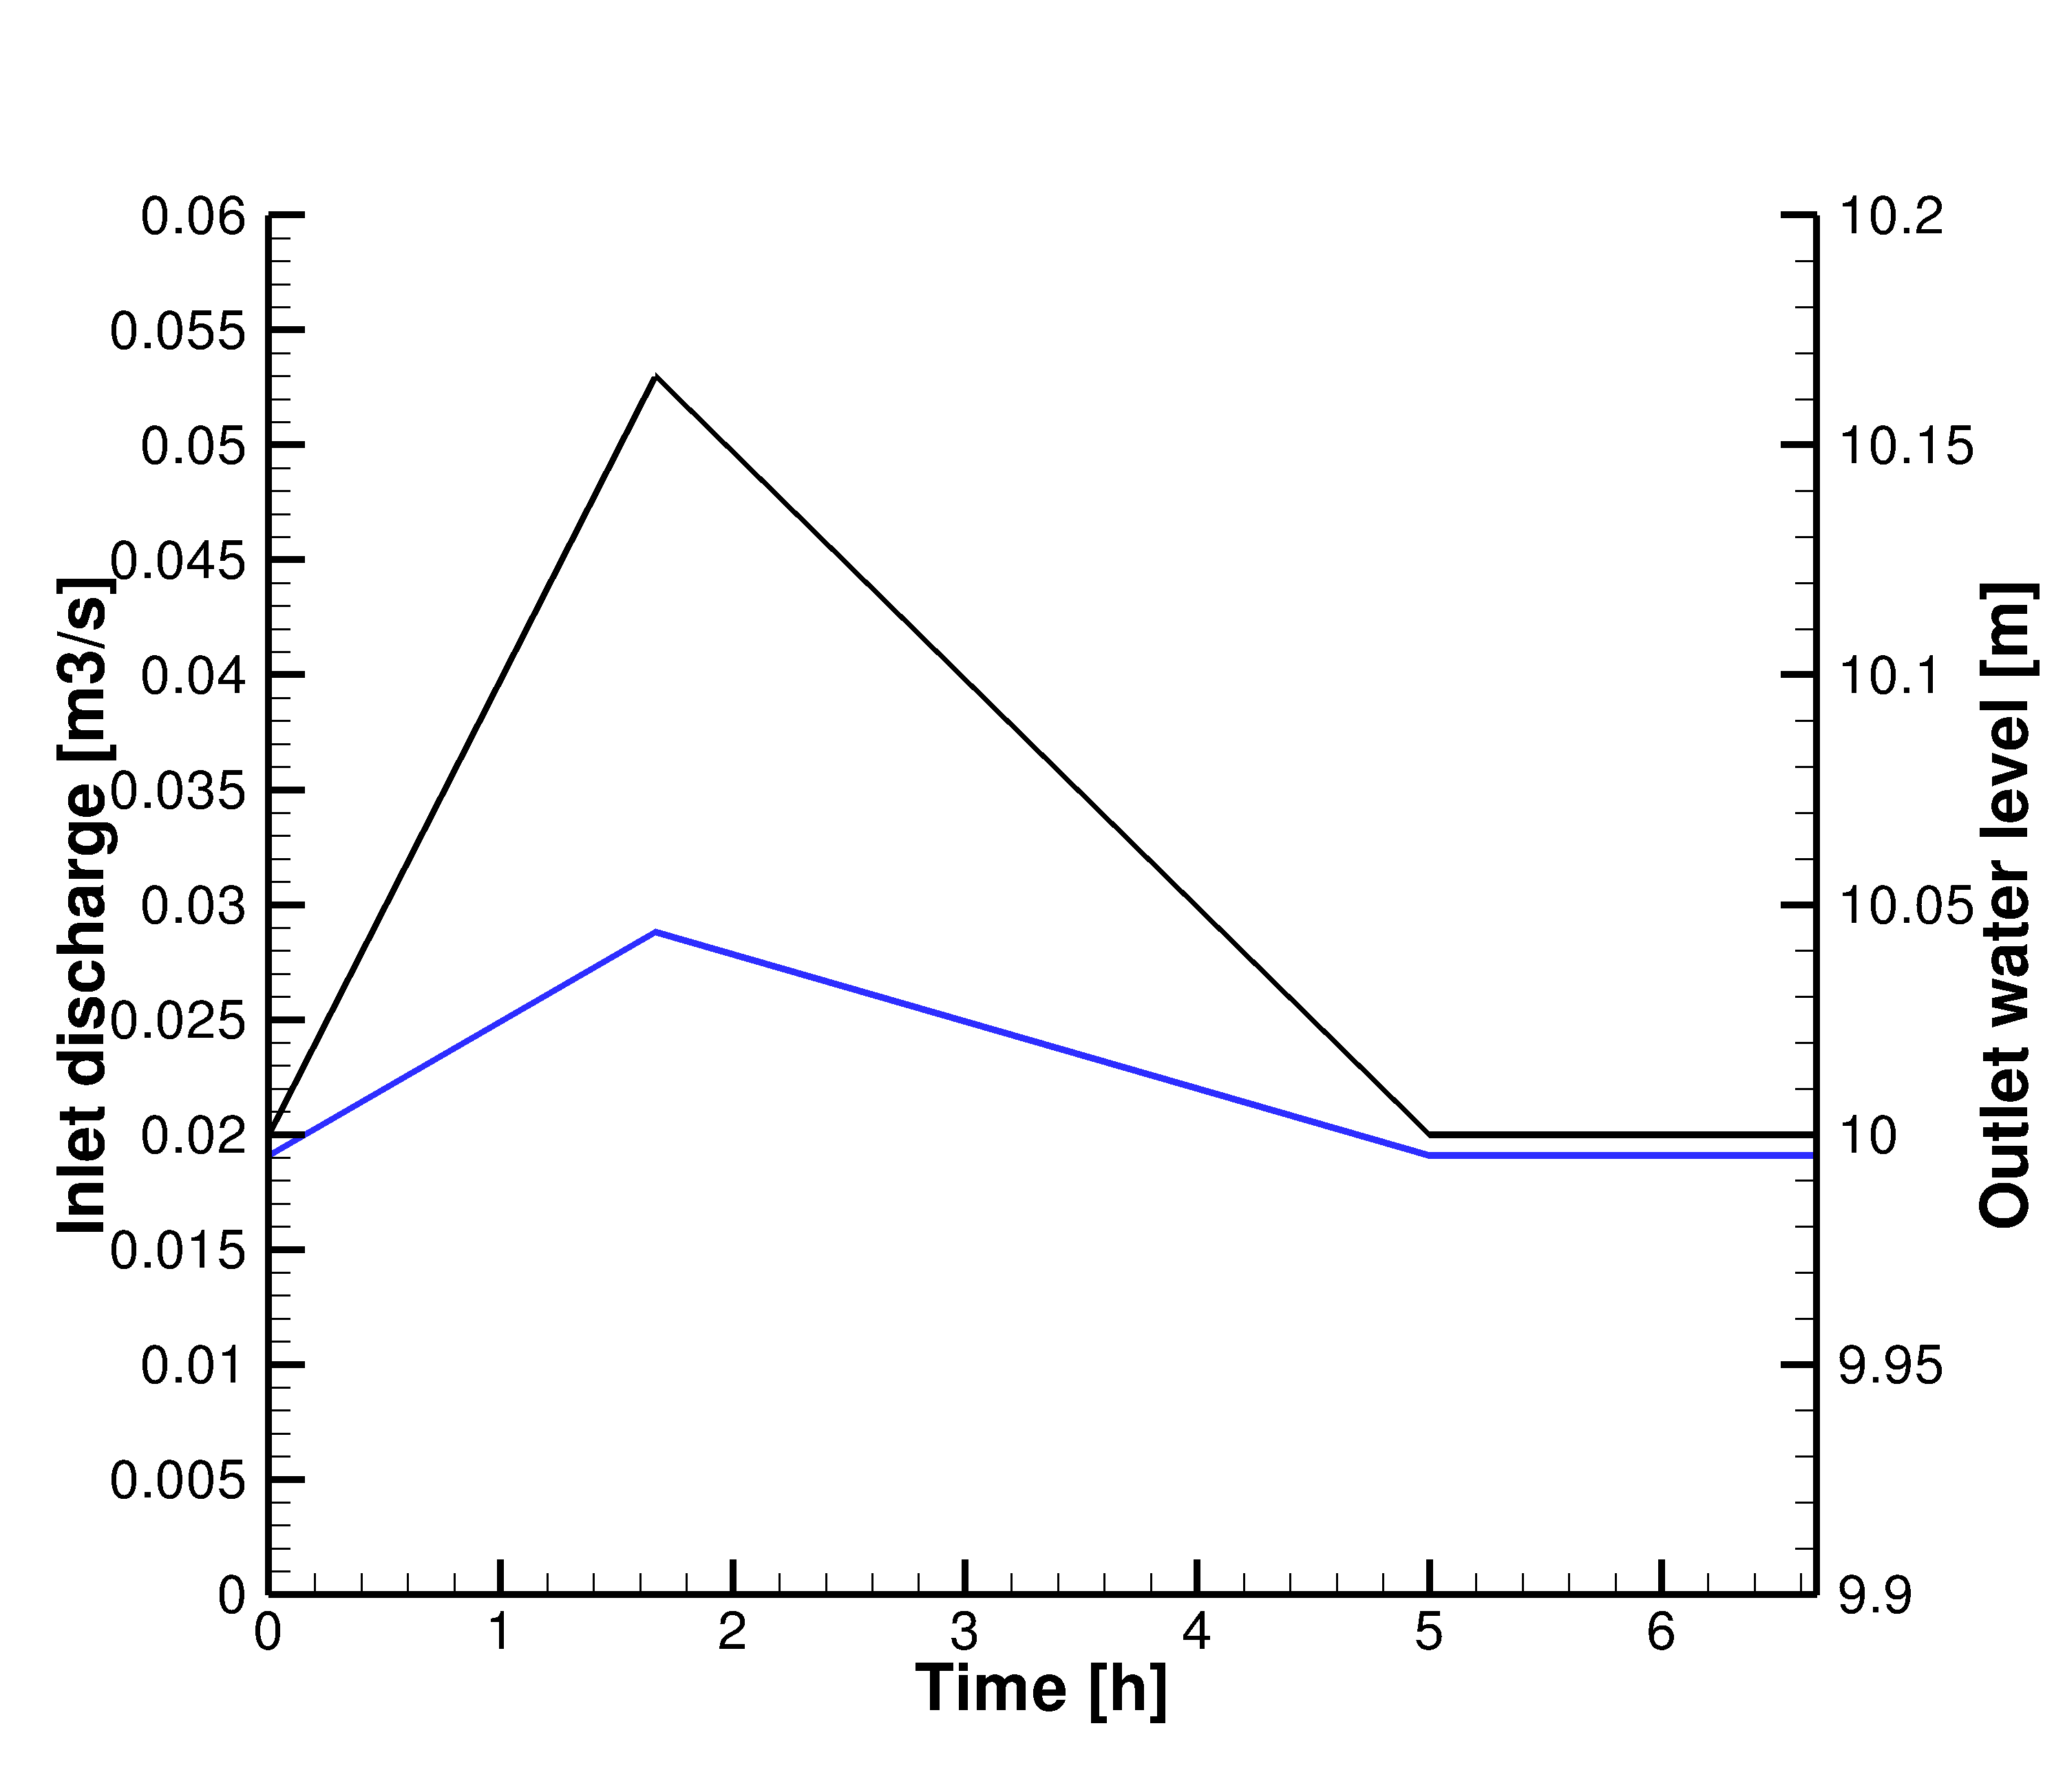
\includegraphics[scale=0.1]{img/yen_boundaries.png}
 \caption{Triangular-shaped hydrograph.}\label{fig:hydro}
\end{figure}

A friction closure relationship, based on the Nikuradse roughness length is adopted to
account for the bed resistance. For this case, $k_s=3.5$ mm ($\approx 3\times D_{50}$) and the Elder model is specified to parameterize the turbulent eddy viscosity.
The critical Shields parameter is set at $0.047$ and the bed porosity is $0.375$.


% - Reference:
%     This part gives the reference solution we are comparing to and
%     explicits the analytical solution when available;
%
%
\section{Numerical setup}
%
Numerical simulations were conducted on an unstructured, triangular finite element mesh with
$3230$ elements and $1799$ nodes and a mean grid size of the order of $0.20$ m (Figure~\ref{fig:mesh}).
As initial condition, a fully developed (stationary) flow with a constant water-depth $h = 0.0544$m and discharge $0.02$ m$^3/$s is imposed and the bottom has a constant slope in flow direction equal to $0.002$.

\begin{figure} [!h]
\centering
  \includegraphicsmaybe{[width=0.6\textwidth]}{../img/bottom.png}
 \caption{Simulation grid and initial bottom.}\label{fig:mesh}
\end{figure}

The time step is set to $0.5$ s. For a mean velocity in the range $[0.37-0.53]$ m/s and
a mean grid size of the order of $0.2$ m, the mean Courant number varies between $0.6$ and $1.3$.

For a daily validation the duration is limited to 2 hours instead of 5 hours.

\section{Results}
%
The measurements were done after 5 hours but for the daily validation the simulation duration was decreased to 2 hours. For a proper comparison the simulation duration must be increased to 5 hours as well.
Numerical results of the normalized bed evolution are shown in
comparison with measurements.
Morphological changes exhibit the expected
patterns of erosion and sedimentation at the channel bend, with the presence of a point bar along the inner-bank and a deeper channel along the outer-bank of the bend.
The computed bed changes are in agreement with the measured data. Without accounting for the secondary flow effect, one cannot obtain such reasonable results.
The subsequent Figures, from \ref{fig:results} to \ref{fig:results_multi3} show the most up to date results with all tested configurations with \gaia.
%The python script compared measurements and simulation at both cross sections.
%One simulated bottom evolution after 5 hours can be seen in figure XXXXX

\begin{figure} [!h]
\centering
\includegraphicsmaybe{[scale=0.35]}{../img/90.png}
\includegraphicsmaybe{[scale=0.35]}{../img/180.png}
\caption{Comparison of simulated and measured normalised bed evolution at cross sections 90$^{\circ}$ (left) and 180$^{\circ}$ (right), with uniform sediment and the Engelund-Hansen \& Chollet-Cunge formula for bedload using Finite Elements (vnv 1) and Finite Volumes (vnv 1 vf) and Meyer-Peter Müller formula with 3 different slope effect formulas (vnv slope1, vnv slope2, vnv slope3).}\label{fig:results}
\end{figure}

\begin{figure} [!h]
\centering
\includegraphicsmaybe{[scale=0.2]}{../img/gaia_yen-exp_EvolutionR04.png}
\includegraphicsmaybe{[scale=0.2]}{../img/gaia_yen-exp_multi3_EvolutionR04.png}
\caption{Comparison of simulated (coloured) and measured (black contour lines) normalised bed evolution (top)
with one sediment class and the Engelund-Hansen \& Chollet-Cunge
  formula for bedload with uniform sediments (left) and with 5 sediment classes (right).}\label{fig:results_vf}
\end{figure}

\begin{figure} [!h]
\centering
\includegraphicsmaybe{[scale=0.35]}{../img/90_multi.png}
\includegraphicsmaybe{[scale=0.35]}{../img/180_multi.png}
\caption{Comparison of simulated normalised bed evolution at cross sections 90$^{\circ}$ (left) and 180$^{\circ}$ (right),
with five sediment classes and different bedload formulas (multi1-multi10).}\label{fig:results_multi1}
\end{figure}

\begin{figure} [!h]
\centering
\includegraphicsmaybe{[scale=0.35]}{../img/90_multi1.png}
\includegraphicsmaybe{[scale=0.35]}{../img/180_multi1.png}
\caption{Comparison of simulated normalised bed evolution at cross sections 90$^{\circ}$ (left) and 180$^{\circ}$ (right),
  with five sediment classes and different Meyer-Peter und Müller bed load formula and different hiding formulas (multi1 hid1 - multi1 hid4).}
\label{fig:results_multi2}
\end{figure}

\begin{figure} [!h]
\centering
\includegraphicsmaybe{[scale=0.15]}{../img/gaia_yen-exp_multi1_EvolutionR04.png}
\includegraphicsmaybe{[scale=0.15]}{../img/gaia_yen-exp_multi2_EvolutionR04.png}
\includegraphicsmaybe{[scale=0.15]}{../img/gaia_yen-exp_multi3_EvolutionR04.png}
\includegraphicsmaybe{[scale=0.15]}{../img/gaia_yen-exp_multi30_EvolutionR04.png}
\includegraphicsmaybe{[scale=0.15]}{../img/gaia_yen-exp_multi4_EvolutionR04.png}
\includegraphicsmaybe{[scale=0.15]}{../img/gaia_yen-exp_multi5_EvolutionR04.png}
\includegraphicsmaybe{[scale=0.15]}{../img/gaia_yen-exp_multi6_EvolutionR04.png}
\includegraphicsmaybe{[scale=0.15]}{../img/gaia_yen-exp_multi7_EvolutionR04.png}
\includegraphicsmaybe{[scale=0.15]}{../img/gaia_yen-exp_multi9_EvolutionR04.png}
\includegraphicsmaybe{[scale=0.15]}{../img/gaia_yen-exp_multi10_EvolutionR04.png}
\caption{Comparison of simulated (coloured) and measured (black contour lines) normalised bed evolution with five sediment classes and different bedload formulas (multi1-multi10).}\label{fig:results_multi3}
\end{figure}


\section{References}
%
Yen, C. and Lee, K.T. (1995) \textit{ Bed Topography and Sediment Sorting in Channel Bend
with Unsteady Flow}. Journal of Hydraulic Engineering, Vol.121, No. 8.
